\section{拉普拉斯谱与生成树}
\label{sec:graph-matrix-tree}

第~\ref{sec:graph-laplacian-eigenvalues}节利用拉普拉斯矩阵的零特征值重数刻画了图的连通分量个数：正权支撑连通（即图中至少存在一棵正权生成树）当且仅当$\lambda_2>0$。本节进一步展示，拉普拉斯矩阵的主余子式以及除去一个零特征值后的$n-1$个特征值$\lambda_2,\ldots,\lambda_n$的乘积，能够精确数出一张图共有多少棵不同的生成树（在加权图中，给出所有生成树的边权乘积之和）。

在四点五边算例中，同样是从五条边中选出三条边，选$\{12,23,34\}$得到一条经过全部四个顶点的无环路径（是生成树），而选$\{12,23,13\}$则把三条边全用在三角形上、遗漏了顶点$4$（不是生成树，见图~\ref{fig:laplacian-tree-minors}）。要理解拉普拉斯矩阵为何能自动筛除所有含环边集、只保留生成树，我们按四个步骤推进：先分析约化关联矩阵的$(n-1)$阶子式如何区分生成树与含环边集，再结合 Cauchy--Binet 公式证明用主余子式计数生成树的矩阵树定理，接着通过特征多项式建立生成树计数的拉普拉斯谱公式，最后代入完全图的拉普拉斯谱导出经典的 Cayley 公式。

\subsection{生成树的关联子式}
\label{sec:graph-tree-incidence-minors}

固定一个顶点$r$作为根，从关联矩阵$\bm B$中删去第$r$行，得到$(n-1)\times m$的约化关联矩阵$\overline{\bm B}$。它仍保留全部$m$条边的列。然后按边序选择$n-1$条边组成集合$S$，只取这些边对应的列，得到$(n-1)\times(n-1)$的方阵$\overline{\bm B}_{:,S}$。

为什么可以删去根的那一行？因为$\bm B$的任一条边的列在两个端点分别取$+1$和$-1$，其余为$0$，所以$\bm B$的各行相加为零向量。一旦其余$n-1$行确定了，根行的值也由零和条件唯一确定。删去根行不会丢失信息。

\begin{lemma}[生成树的关联子式]
\label{lem:graph-tree-incidence-minors}
若$S$构成生成树，则$\det(\overline{\bm B}_{:,S})\in\{1,-1\}$。其他含$n-1$条边的集合$S$都使该行列式为零。
\end{lemma}

\begin{proof}
先处理$S$含环的情形。沿环选定一个行走方向，对每条环边，如果行走方向与记录方向一致就取原列，否则取负列。调整后，每列把环的上一步端点标为$+1$、下一步端点标为$-1$。

环上的任何一个顶点都在两条环边上出现：从进入的边收到$-1$，从离开的边收到$+1$，两者抵消为零。把调整后的列全部加起来，得到零向量。删去根行后仍然是零。这说明列之间有线性关系，行列式为零。

再处理$S$不含环的情形。$n$个顶点和$n-1$条无环边构成一个森林。设森林有$c$个连通分量，其中每棵树的顶点数比边数多一，因此总共有$n-c$条边。我们选了$n-1$条边，所以$c=1$，这组边构成一棵生成树。

对生成树，我们用递归计算它的关联子式。树中至少有两个顶点，就可以找到一个不是根的叶顶点。叶在生成树中只连一条边，因此$\overline{\bm B}_{:,S}$中对应的行只有一个非零条目，值为$+1$或$-1$。

沿这一行展开行列式，去掉叶所在的行和叶边所在的列，剩余矩阵是较小的树删去根行后的关联矩阵。每次展开只乘一个$\pm1$的因子。反复删去非根叶，最后只剩根，而根行在开始时已经删去，此时是一个空矩阵，行列式约定为$1$。逐层回乘，原行列式的绝对值为$1$。
\end{proof}

在四点算例中删去第$4$行。取边集$\{12,23,34\}$得到
\[
  \overline{\bm B}_{:,\{12,23,34\}}=
  \begin{bmatrix}
  1&0&0\\
  -1&1&0\\
  0&-1&1
  \end{bmatrix}.
\]
这是对角线全为$1$的下三角矩阵，行列式为$1$。改选$\{12,23,13\}$，由于这三条边构成三角形$1\!-\!2\!-\!3$，环的线性关系使行列式为零。后一组虽然也是三条边，却遗漏了顶点$4$。

图~\ref{fig:laplacian-tree-minors}把两种选法并排展示。左图中的边$34$经过根顶点$4$，但它的列仍然保留——删去的只是根对应的行，不影响边的列。

\begin{BookInlineFigure}
  \centering
  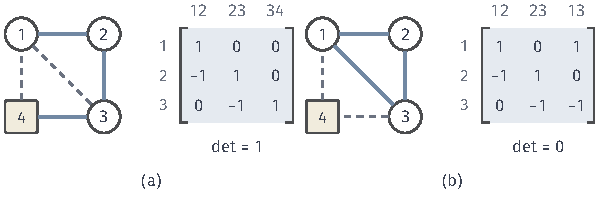
\includegraphics{figures/03-graphs/05-matrices-and-spectra/tikz/laplacian-tree-minors.pdf}
  \caption{固定根$4$后对照两组边的关联子式。方框标出根，它没有对应的矩阵行。实线表示选中的边，同时给出矩阵的列标。（a）生成树的子式行列式为一。（b）三角形的子式前两列相加等于第三列。}
  \label{fig:laplacian-tree-minors}
\end{BookInlineFigure}

\subsection{生成树的代数余子式计数}
\label{sec:graph-matrix-tree-proof}

现在把约化关联子式的判别性质与\BookChapterRef{chap:linear-operations}{卷二“向量、矩阵与张量的运算”章}的 Cauchy--Binet 公式结合起来，导出用拉普拉斯矩阵的代数余子式计数生成树的矩阵树定理。

从组合拉普拉斯矩阵$\bm L$中删去第$r$行和第$r$列，得到$(n-1)\times(n-1)$主子矩阵$\overline{\bm L}=\bm L^{(r,r)}$，其行列式$\det\overline{\bm L}=(-1)^{r+r}\det\bm L^{(r,r)}$正是对角位置$(r,r)$处的代数余子式$C_{r,r}$。

由关联分解式~\eqref{eq:graph-laplacian-incidence-factorization}，$\overline{\bm L}$的每个条目为
\[
  \overline L_{i,j}=\sum_{e\in E} B_{i,e}\,w_e\,B_{j,e},
\]
其中$i,j$遍历除$r$以外的$n-1$个顶点，求和仍遍及全部$m$条边。因此可以用$(n-1)\times m$约化关联矩阵$\overline{\bm B}$写成
\[
  \overline{\bm L}=\overline{\bm B}\,\bm C\,\overline{\bm B}^\top.
\]

进一步令$\bm M=\overline{\bm B}\bm C^{1/2}\in\mathbb R^{(n-1)\times m}$，使$\bm M$的每列为原来的约化关联列乘以该边权重的平方根$\sqrt{w_e}$。于是主子矩阵分解为
\[
  \overline{\bm L}=\bm M\bm M^\top,
\]
这正是 Cauchy--Binet 公式适用的矩形矩阵乘积形式。

\begin{theorem}[矩阵树定理]
\label{thm:graph-matrix-tree}
对有限无向非负权图，设$\mathcal T$为图的所有生成树的集合。则组合拉普拉斯矩阵$\bm L$在任意位置$(i,j)$处的代数余子式$C_{i,j}=(-1)^{i+j}\det\bm L^{(i,j)}$（特别地，删去任一顶点$r$的第$r$行与第$r$列所得的主余子式$\det\overline{\bm L}$）全部相等，且\term{矩阵树定理}（matrix-tree theorem）给出
\begin{equation}
  \det \overline{\bm L}=(-1)^{i+j}\det\bm L^{(i,j)}=\sum_{T\in\mathcal T}\prod_{e\in T}w_e.
  \label{eq:graph-matrix-tree}
\end{equation}
单位权时每棵生成树贡献$1$，该代数余子式就是生成树的数目。
\end{theorem}

\begin{proof}
第一步，对$(n-1)\times m$矩阵$\bm M$与$m\times(n-1)$矩阵$\bm M^\top$的乘积$\overline{\bm L}=\bm M\bm M^\top$应用 Cauchy--Binet 公式（参见\BookChapterRef{chap:linear-operations}{卷二“向量、矩阵与张量的运算”章}）。每次从$m$列中选出$n-1$个列指标（即选出一个$n-1$元边集$S\subseteq E$），由于$(\bm M^\top)_{S,:}=(\bm M_{:,S})^\top$，对应行和对应列组成的两个$(n-1)$阶子方阵互为转置、行列式相等，故
\[
  \det\overline{\bm L}
  =\sum_{\substack{S\subseteq E\\ |S|=n-1}}\det(\bm M_{:,S})\det\bigl((\bm M^\top)_{S,:}\bigr)
  =\sum_{\substack{S\subseteq E\\ |S|=n-1}}\det(\bm M_{:,S})^2.
\]

第二步，提取每条边的权重因子。$\bm M$的第$e$列是$\overline{\bm B}$的第$e$列乘以$\sqrt{w_e}$。取出$S$中各列后，由行列式对各列的齐次性，每列各提出一个$\sqrt{w_e}$因子，平方后变成$w_e$，因此
\[
  \det(\bm M_{:,S})^2=\det(\overline{\bm B}_{:,S})^2\prod_{e\in S}w_e.
\]

第三步，代入关联子式的判别结果。由引理~\ref{lem:graph-tree-incidence-minors}，如果$S$构成生成树，关联子式$\det(\overline{\bm B}_{:,S})$为$\pm1$，平方为$1$，该项贡献恰好是这棵生成树各边权重的乘积$\prod_{e\in S}w_e$；如果$S$不是生成树，关联子式为零，该项贡献为零。把所有非零项相加，即得对角位置的主余子式公式$\det\overline{\bm L}=\sum_{T\in\mathcal T}\prod_{e\in T}w_e$。

第四步，证明任意非对角位置$(i,j)$（$i\neq j$）的代数余子式$C_{i,j}=(-1)^{i+j}\det\bm L^{(i,j)}$也等于$\det\bm L^{(i,i)}$。在删去第$i$行与第$j$列所得的$(n-1)$阶子矩阵$\bm L^{(i,j)}$中，原矩阵的第$i$列保留了下来；将$\bm L^{(i,j)}$中除原第$i$列以外的其余$n-2$列全部加到原第$i$列上，行列式不变。由于$\bm L$的每一行元素之和为零（$\bm L\bm 1=\bm 0$），相加后原第$i$列在每一行上的新元素恰好等于$-\bm L^{(i,i)}$中原编号为$j$的列的元素。

最后，通过$|i-j|-1$次相邻列交换，把这一列移到原第$j$列在$\bm L^{(i,i)}$中的位置。列变号与列交换带来的总符号因子为$-(-1)^{|i-j|-1}=(-1)^{i+j}$，与代数余子式定义中的$(-1)^{i+j}$相乘恰好为$+1$，从而$(-1)^{i+j}\det\bm L^{(i,j)}=\det\bm L^{(i,i)}$。
\end{proof}

由于树权总和不涉及任何特定根，删去不同顶点的行列后得到的主余子式全都相等。含零权边的树在乘积中贡献为零；若正权支撑不连通，所有生成树至少包含一条零权边，权积全为零，代数余子式也为零。

下面在四点五边单位权算例上核对。删去顶点$3$对应的行和列，得到$3\times 3$约化矩阵
\[
  \overline{\bm L}=
  \begin{bmatrix}
  3&-1&-1\\
  -1&2&0\\
  -1&0&2
  \end{bmatrix}.
\]
沿第一行展开行列式：
\[
  \begin{aligned}
    \det\overline{\bm L}
    &=3\cdot\det\begin{bmatrix}2&0\\0&2\end{bmatrix}
      -(-1)\cdot\det\begin{bmatrix}-1&0\\-1&2\end{bmatrix}
      +(-1)\cdot\det\begin{bmatrix}-1&2\\-1&0\end{bmatrix}\\
    &=3\times 4 + 1\times(-2) - 1\times 2 = 12-2-2=8.
  \end{aligned}
\]

从组合计数看，五条边任选三条共有$\binom53=10$组。其中两个三角形$\{12,23,13\}$与$\{13,34,41\}$各自成环，贡献为零；其余$8$组各构成一棵生成树，单位权下各贡献$1$，总数为$8$。

若将对角边$13$的权重改为$2$，生成树的集合本身不变，但每棵包含边$13$的生成树权积变为$2$。含边$13$的生成树还需将顶点$2$和$4$分别接入$\{1,3\}$：顶点$2$可选边$12$或$23$（$2$种），顶点$4$可选边$34$或$41$（$2$种），共$2\times 2=4$棵。这$4$棵树各贡献$2$，其余$4$棵不含边$13$的树各贡献$1$，加权生成树总和变为$4\times 2+4\times 1=12$。

\subsection{生成树的拉普拉斯谱公式}
\label{sec:graph-tree-counting-formulas}

矩阵树定理把生成树权重总和表示为删去任一顶点行列所得的主余子式$\det\overline{\bm L}$。将全部$n$个顶点的主余子式汇总到$\bm L$的特征多项式一次项系数中，就可以直接用拉普拉斯矩阵的其余$n-1$个特征值$\lambda_2,\ldots,\lambda_n$表达生成树权重总和。

\begin{theorem}[生成树计数的拉普拉斯谱公式]
\label{cor:graph-tree-count-spectrum}
设$n\geq 2$，有限无向非负加权图的组合拉普拉斯特征值按升序排列为$0=\lambda_1\leq\lambda_2\leq\cdots\leq\lambda_n$。则图的生成树权重总和满足
\begin{equation}
  \sum_{T\in\mathcal T}\prod_{e\in T}w_e
  =\frac1n\prod_{i=2}^n\lambda_i.
  \label{eq:graph-tree-count-from-spectrum}
\end{equation}
\end{theorem}

\begin{proof}
第一步，从特征值展开计算$\det(t\bm I+\bm L)$中$t$的一次项系数。在$\bm L$的正交特征基下，$t\bm I+\bm L$的特征值为$t+\lambda_1,\ldots,t+\lambda_n$；因$\lambda_1=0$，有
\[
  \det(t\bm I+\bm L)=t\prod_{i=2}^n(t+\lambda_i).
\]
将其按$t$的幂展开，$t$的一次项系数为$\prod_{i=2}^n\lambda_i$。

第二步，从行列式按列的多线性计算同一系数。将$\det(t\bm I+\bm L)$的第$r$列写成$t\bm e_r + \bm L_{:,r}$；展开式中含$t$的一次项恰好来自“在某一列$r$选取$t\bm e_r$、在其余$n-1$列选取$\bm L$的原列”的所有组合。对固定的$r\in\{1,\ldots,n\}$，将第$r$列替换为$t\bm e_r$后沿第$r$列作拉普拉斯展开，所得$t$的系数正是删去$\bm L$的第$r$行与第$r$列后的主余子式$\det\overline{\bm L}^{(r)}$。

第三步，应用矩阵树定理求并比较系数。由定理~\ref{thm:graph-matrix-tree}，每个顶点$r$的主余子式均等于$\sum_{T\in\mathcal T}\prod_{e\in T}w_e$。对$r=1,\ldots,n$求和，可知$\det(t\bm I+\bm L)$中$t$的一次项系数又等于$n\sum_{T\in\mathcal T}\prod_{e\in T}w_e$。比较两种展开的一次项系数并除以$n$，即得式~\eqref{eq:graph-tree-count-from-spectrum}。
\end{proof}

在四点五边单位权算例中，第~\ref{sec:graph-laplacian-frequency}小节已算出$\bm L$的四个特征值为$0,2,4,4$。代入式~\eqref{eq:graph-tree-count-from-spectrum}得
\[
  \frac{1}{4}\times(2\times 4\times 4)=8,
\]
与上一小节直接展开$3\times 3$约化行列式所得的$8$棵生成树完全一致。

此外，若将全图所有边权同时乘以正数$a>0$，每棵生成树包含$n-1$条边，其边权乘积乘以$a^{n-1}$；与此同时，每个非零特征值$\lambda_i$也乘以$a$，式~\eqref{eq:graph-tree-count-from-spectrum}右侧$n-1$个特征值之积同样乘以$a^{n-1}$，两端具有相同的齐次尺度。

\subsection{完全图的Cayley公式}
\label{sec:graph-cayley-formula}

将第~\ref{sec:graph-typical-laplacian-spectra}小节求出的典型图拉普拉斯谱代入定理~\ref{cor:graph-tree-count-spectrum}，无需再逐个展开行列式，就能直接算出图族的生成树数目。其中最著名的应用是完全图$K_n$的生成树计数——由于$K_n$包含$n$个标号顶点之间的全部可能连边，$K_n$的生成树与$n$个标号顶点上的所有标号树一一对应。

\begin{theorem}[Cayley公式]
\label{thm:graph-cayley-formula}
设$n\geq 2$。单位权完全图$K_n$的生成树个数（即$n$个标号顶点上的标号树总数）满足\emph{Cayley公式}（Cayley's formula）：
\begin{equation}
  |\mathcal T(K_n)|=n^{n-2}.
  \label{eq:graph-cayley-count}
\end{equation}
\end{theorem}

\begin{proof}
由定理~\ref{prop:graph-typical-laplacian-spectra}，单位权完全图$K_n$的组合拉普拉斯谱为$\lambda_1=0$（重数$1$）与$\lambda_2=\cdots=\lambda_n=n$（重数$n-1$）。代入谱公式~\eqref{eq:graph-tree-count-from-spectrum}，立得
\[
  |\mathcal T(K_n)|=\frac{1}{n}\prod_{i=2}^n n=\frac{1}{n}\cdot n^{n-1}=n^{n-2}.
\]
\end{proof}

也可以直接在约化矩阵上核对完全图的 Cayley 公式：从$\bm L(K_n)=n\bm I_n-\bm 1_n\bm 1_n^\top$中删去一行一列后，$(n-1)\times(n-1)$约化矩阵为$\overline{\bm L}=n\bm I_{n-1}-\bm 1_{n-1}\bm 1_{n-1}^\top$。该矩阵在全一向量$\bm 1_{n-1}$方向上的特征值为$n-(n-1)=1$，在正交补上的$n-2$个特征值仍为$n$，特征值乘积同样给出$\det\overline{\bm L}=1\cdot n^{n-2}=n^{n-2}$。

用同样的方法核对星图$K_{1,n-1}$：由定理~\ref{thm:graph-star-laplacian-spectrum}知其非零拉普拉斯特征值为$n-2$个$1$和$1$个$n$，代入式~\eqref{eq:graph-tree-count-from-spectrum}得$|\mathcal T(K_{1,n-1})|=\frac{1}{n}(1^{n-2}\cdot n)=1$，与树本身只有唯一一棵生成树一致。
